%------------------------------------------------------------
%
\documentclass{exam}
%

\usepackage{amsmath}%
\usepackage{amsfonts}%
\usepackage{amssymb}%
\usepackage{fullpage}
\usepackage{graphicx}
%\usepackage{setspace}
%\usepackage{float}
\usepackage{hyperref}
\usepackage{tikz}
\usepackage{xcolor}
\usepackage[normalem]{ulem}
\usepackage[outline]{contour}
\usepackage{subcaption}
\usepackage{multirow}

%\renewcommand*{\theenumi}{\thesection.\arabic{enumi}}
\newcommand{\BE}{\begin{equation}}
\newcommand{\EE}{\end{equation}}
\newcommand{\BEBA}{\begin{equation}\begin{aligned}}
\newcommand{\EAEE}{\end{aligned}\end{equation}}

\newcommand{\firstDueDate}{Sept. 15}
\newcommand{\secondDueDate}{Oct. 1}
\newcommand{\thirdDueDate}{Oct. 15}
\newcommand{\fourthDueDate}{Nov. 1}
\newcommand{\fifthDueDate}{Nov. 15}
\newcommand{\methodsDueDate}{Nov. 15}
\newcommand{\finalDueDate}{Dec. 1}
\newcommand{\integrityLink}{\url{https://stedwards.app.box.com/s/izo4b4q9hywr5bfiq93ll4s8bls69rk1}}
\newcommand{\DSTstart}{Mar. 10}
\newcommand{\DSTend}{Nov. 3}




\title{Moon Project}
\date{}
\begin{document}
\maketitle
The semester long project will require you to record of the position and appearance of the Moon in the sky, then use this information to find the how long the Moon takes to orbit the Earth relative to the Sun, and to predict the phase of the Moon.


\section{Due Dates}
You will turn in observations over the course of the semester. Each time you turn the project in you must have at least four new observations. The dates are\\
\begin{table}[!h]
\centering
\begin{tabular}{|l|l|}
\hline
First Observations & \firstDueDate\\
Second Observations & \secondDueDate\\
Third Observations & \thirdDueDate\\
Fourth Observations & \fourthDueDate\\
Fifth Observations & \fifthDueDate\\
Methods Write-Up & \methodsDueDate\\
Final Observations \& Write-up & \finalDueDate\\
\hline
\end{tabular}
\end{table}

The Methods Write-Up is a chance for you to submit a sample of your writing and get feedback before the final project is due.

\section{Academic Integrity}
You are allowed to discuss your work with other students in the class to understand the concepts and methods used to solve problems or do the analysis. Each student is expected to do and present their own work and be respectful to other students in the class. 

Plagiarism, cheating, and falsifying data will not be tolerated. The codes for student conduct, academic integrity, and plagiarism can be found at\\ \integrityLink. All incidents of academic dishonesty will be brought to the attention of Dean of Students Office and may be subject to academic penalties commensurate with the severity of the offense.

\textbf{Any observation that is deemed to be falsified will not be accepted and is likely to result in a referral to the Dean of Students.}


\section{Grading}
The grading for the project is broken down in Table \ref{tab:grading}. Note that the numbers do add up to more than 100\%. With every possible observation, %and doing the Length of Day portion,
you could have a score of up to about 125\%, meaning you get 25\% extra credit.

\begin{table}[!h]
\centering
\begin{tabular}{|ll|}
\hline
Each set of observations & 7.5\% (minimum of 2${}^*$)\\
& 0.5\% for each additional observation${}^*$\\
Methods Write-Up   & 5\%\\
Final Project Write-Up   & 50\%\\
%Length of Day on the Moon (optional) & 5\% (extra credit)\\
\hline
\multicolumn{2}{p{14cm}}{${}*$ Observations must be made at least 18 hours apart (i.e. you won't get credit for multiple observations on the same day).}\\
\end{tabular}
\caption{\label{tab:grading}Grade components for the project}
\end{table}

\section{Project Write-Up}
The write-up should be presented as if it were a scientific paper or lab write-up. The sections and descriptions are listed in Table \ref{tab:writeup}.
\begin{table}[!h]
\centering
\begin{tabular}{|lp{11cm}|}
\hline
\textbf{Title} & A brief description of the work that is understandable by someone not in the class.\\
\textbf{Introduction} & A short description of the motiviation of the work and an explanation of any terms or concepts that the reader needs in order to understand the work.\\
\textbf{Methods} & An explanation of how you took your measurements. This should be written so that a person not taking the class could understand how you measured the Moon's position.\\
\textbf{Results} \& Analysis & Here you present the findings based on your observations. Specifically, you want to identify the period, relationship between phase, period, and elongation, and what you find for the length of day for the Moon. You do not need to include a list of all observations; but some form of graph that demonstrates your results should be included. The graph cannot be stand-alone; the text should refer to any graphs and discuss what you want the reader to notice, and account for any unusual variations or deficiencies in the plot (e.g. large gaps in data, data outliers, etc.).\\
\textbf{Discussion} & Discuss the implications of the results and the methods that you used. Can the methods be used for other things? What uncertainties or biases might there be in your methods? How might you perform this projet to improve the uncertainty. How do your results compare to the `known' values?\\
\textbf{Conclusion} & Summarize the purpose, methods, and results, limitations, or future value of your work. \\
\hline
\end{tabular}
\caption{\label{tab:writeup}The sections that should be in the write-up}
\end{table}
\section{Rubric for Write-Up}
The final write-up is graded based on writing and content. The weights and details are listed in Table \ref{tab:rubric}.

\begin{table}[!h]
\centering
\begin{tabular}{|c|c|p{6.25cm}|c|}
\hline
Section & Item & Criterion & Weight\\
\hline
\hline
Introduction        & Motivation & Provides a clear explanation for the project & 5\\
                    & Background & Provides necessary background to support motivation and explain concepts to be used in the report & 5\\
\hline
Methods             &            & Describes the methodology used to take observations & 10\\
\hline
Results \& Analysis & Period (graph)     & Shows a graph with results that are used to find the period of the orbit & 5\\
                    & Period (text)      & Describes in the text how the period is found from the graph. Gives the value that is found in the experiment & 5\\
                    & Phase vs. elongation (graph) & Shows a graph that demonstrates the relation between the phase and the elongation & 5\\
                    & Phase vs. elongation (text)  & Describes within the text the relation between phase and elongation. & 5\\
\hline
Discussion          & Comparison         & Compares the results with data from other sources & 5\\
                    & Uncertainty analysis & Addresses limitations of the methods used. Describes uncertainty in the results due to the limitations & 5\\
                    & Other limitations  & Addresses any other uncertainties or limitations in the data & 5\\
\hline
Conclusion          & Summary           & Summarizes final results & 5\\
                    & Discussion        & Describes relevance of results & 5\\
\hline
Writing             & Spelling \& Mechanics & Writing is free from spelling errors, has correct punctuation, etc. & 5\\
                   & Grammar & Writing is grammatically correct & 5\\
                  & Concision & Writing is concise yet provides all necessary details & 5\\
                   & Clarity & Writing is clear and easy for a college-educated reader to understand & 10\\
                   & References \& Bibliography & All required citations and bibliography are included (if relevant) & 5${}^*$\\
                   & Own Work   & All writing is the author's own work or is otherwise cited                         & 5${}^*$ \\
\hline
\multicolumn{4}{p{14cm}}{* --- Intentional plagiarism will not be tolerated and will result in a 0 and referral to the Dean of Students.  A significant lack of required citations may result in a loss of more than 5 points.}
\end{tabular}
\caption{\label{tab:rubric} Rubric for write-up.}
\end{table}
\newpage


\section{Finding the Period}
To find the period of the Moon's orbit, you will need to create a graph showing the relation between elongation and time since first observation. The elongation is limited to $0$ -- $360^\circ$, so when the elongation would go from say 359° to 360° it instead wraps back to 0°. For example, if you had the data listed in Table \ref{Tab:elongation} for time and elongation, Figure \ref{fig:days_elongation_data_only} demonstrates what the plot would look like. In this case, since the elongation keeps wrapping back to 0°, the pattern it makes is like a sawtooth.
\begin{table}[!h]
\centering
\begin{tabular}{|c|c|c||c|c|c|}
\hline
 		& Time 			&   			&  		& Time 			&   			\\
 		& since 		&   			&  		& since 		&   			\\
 		& first  		&   			&  		& first  		&   			\\
 		& observation  	& Elongation  	&  		& observation  	& Elongation  	\\
Date 	& (days) 		& (°)  			& Date 	& (days) 		& (°)  			\\
\hline
Dec 26 & 0 & 220 & Jan 27 & 32 & 254 \\
Jan 02 & 7 & 303 & Jan 31 & 36 & 329 \\
Jan 03 & 8 & 322 & Feb 05 & 41 & 37 \\
Jan 08 & 13 & 41 & Feb 10 & 46 & 85 \\
Jan 09 & 14 & 66 & Feb 13 & 49 & 153 \\
Jan 12 & 17 & 54 & Feb 18 & 54 & 229 \\
Jan 15 & 20 & 112 & Feb 19 & 55 & 227 \\
Jan 16 & 21 & 165 & Feb 23 & 59 & 304 \\
Jan 18 & 23 & 156 & Feb 26 & 62 & 332 \\
Jan 19 & 24 & 152 & Mar 02 & 66 & 1 \\
Jan 20 & 25 & 216 & Mar 07 & 71 & 68 \\
Jan 23 & 28 & 239 & Mar 12 & 76 & 131 \\
Jan 25 & 30 & 277 & Mar 17 & 81 & 211 \\
\hline
\end{tabular}\\
\caption{\label{Tab:elongation}A set of observations of the Moon showing the time since the first observation and the observed elongation on each date.}
\end{table}




\begin{figure}[!h]
\centering
\begin{subfigure}[t]{0.48\textwidth}
\centering
\begin{tikzpicture}
\draw[black, line width=0.25mm, ->] (0.0,0) -- (0.0,\linewidth*0.76*0.7692);
\draw[black, line width=0.25mm, ->] (0.0,0) -- ({\linewidth*0.76},0);
\draw[black] (0,0) -- ++(0.0,-0.25) node[below] {0};
\draw[black] ({15.0/90.0*\linewidth*0.76},0) -- ++(0.0,-0.25) node[below] {15};
\draw[black] ({30.0/90.0*\linewidth*0.76},0) -- ++(0.0,-0.25) node[below] {30};
\draw[black] ({45.0/90.0*\linewidth*0.76},0) -- ++(0.0,-0.25) node[below] {45};
\draw[black] ({60.0/90.0*\linewidth*0.76},0) -- ++(0.0,-0.25) node[below] {60};
\draw[black] ({75.0/90.0*\linewidth*0.76},0) -- ++(0.0,-0.25) node[below] {75};
\draw[black] ({90.0/90.0*\linewidth*0.76},0) -- ++(0.0,-0.25) node[below] {90};
\draw[black] (0.0,0) -- ++(-0.25,0) node[left] {0};
\draw[black] (0.0,{60.0 / 360.0*\linewidth*0.76*0.7692}) -- ++(-0.25,0) node[left] {60};
\draw[black] (0.0,{120.0 / 360.0*\linewidth*0.76*0.7692}) -- ++(-0.25,0) node[left] {120};
\draw[black] (0.0,{180.0 / 360.0*\linewidth*0.76*0.7692}) -- ++(-0.25,0) node[left] {180};
\draw[black] (0.0,{240.0 / 360.0*\linewidth*0.76*0.7692}) -- ++(-0.25,0) node[left] {240};
\draw[black] (0.0,{300.0 / 360.0*\linewidth*0.76*0.7692}) -- ++(-0.25,0) node[left] {300};
\draw[black] (0.0,{360.0 / 360.0*\linewidth*0.76*0.7692}) -- ++(-0.25,0) node[left] {360};
\draw[black] ({-0.18*\linewidth},{0.5*\linewidth*0.76*0.7692}) node[rotate=90] {Elongation [°]};
\draw[black] ({0.5*\linewidth*0.76},{-0.12*\linewidth}) node {Time Since First Observation [days]};
\fill[black] ({0/90*\textwidth*0.76},{220/360*\textwidth*0.76*0.7692}) circle (0.07);
\fill[black] ({7/90*\textwidth*0.76},{303/360*\textwidth*0.76*0.7692}) circle (0.07);
\fill[black] ({8/90*\textwidth*0.76},{322/360*\textwidth*0.76*0.7692}) circle (0.07);
\fill[red] ({13/90*\textwidth*0.76},{41/360*\textwidth*0.76*0.7692}) circle (0.07);
\fill[red] ({14/90*\textwidth*0.76},{66/360*\textwidth*0.76*0.7692}) circle (0.07);
\fill[red] ({17/90*\textwidth*0.76},{54/360*\textwidth*0.76*0.7692}) circle (0.07);
\fill[red] ({20/90*\textwidth*0.76},{112/360*\textwidth*0.76*0.7692}) circle (0.07);
\fill[red] ({21/90*\textwidth*0.76},{165/360*\textwidth*0.76*0.7692}) circle (0.07);
\fill[red] ({23/90*\textwidth*0.76},{156/360*\textwidth*0.76*0.7692}) circle (0.07);
\fill[red] ({24/90*\textwidth*0.76},{152/360*\textwidth*0.76*0.7692}) circle (0.07);
\fill[red] ({25/90*\textwidth*0.76},{216/360*\textwidth*0.76*0.7692}) circle (0.07);
\fill[red] ({28/90*\textwidth*0.76},{239/360*\textwidth*0.76*0.7692}) circle (0.07);
\fill[red] ({30/90*\textwidth*0.76},{277/360*\textwidth*0.76*0.7692}) circle (0.07);
\fill[red] ({32/90*\textwidth*0.76},{254/360*\textwidth*0.76*0.7692}) circle (0.07);
\fill[red] ({36/90*\textwidth*0.76},{329/360*\textwidth*0.76*0.7692}) circle (0.07);
\fill[blue] ({41/90*\textwidth*0.76},{37/360*\textwidth*0.76*0.7692}) circle (0.07);
\fill[blue] ({46/90*\textwidth*0.76},{85/360*\textwidth*0.76*0.7692}) circle (0.07);
\fill[blue] ({49/90*\textwidth*0.76},{153/360*\textwidth*0.76*0.7692}) circle (0.07);
\fill[blue] ({54/90*\textwidth*0.76},{229/360*\textwidth*0.76*0.7692}) circle (0.07);
\fill[blue] ({55/90*\textwidth*0.76},{227/360*\textwidth*0.76*0.7692}) circle (0.07);
\fill[blue] ({59/90*\textwidth*0.76},{304/360*\textwidth*0.76*0.7692}) circle (0.07);
\fill[blue] ({62/90*\textwidth*0.76},{332/360*\textwidth*0.76*0.7692}) circle (0.07);
\fill[orange] ({66/90*\textwidth*0.76},{1/360*\textwidth*0.76*0.7692}) circle (0.07);
\fill[orange] ({71/90*\textwidth*0.76},{68/360*\textwidth*0.76*0.7692}) circle (0.07);
\fill[orange] ({76/90*\textwidth*0.76},{131/360*\textwidth*0.76*0.7692}) circle (0.07);
\fill[orange] ({81/90*\textwidth*0.76},{211/360*\textwidth*0.76*0.7692}) circle (0.07);
\end{tikzpicture}
\caption{\label{fig:days_elongation_data_only}The graph of the elongation vs. time since the first observation. The Moon's elongation transitions from 359° to 0°, causing the plot to look like a sawtooth. The points are color coded to help identify the points in each graph.}
\end{subfigure}
\hfill
\begin{subfigure}[t]{0.48\textwidth}
\centering
\begin{tikzpicture}
\draw[black, line width=0.25mm, ->] (0.0,0) -- (0.0,{\linewidth*0.76*0.7692});
\draw[black, line width=0.25mm, ->] (0.0,0) -- ({\linewidth*0.76},0);
\draw[black] (0,0) -- ++(0.0,-0.25) node[below] {0};
\draw[black] ({15.0/90.0*\linewidth*0.76},0) -- ++(0.0,-0.25) node[below] {15};
\draw[black] ({30.0/90.0*\linewidth*0.76},0) -- ++(0.0,-0.25) node[below] {30};
\draw[black] ({45.0/90.0*\linewidth*0.76},0) -- ++(0.0,-0.25) node[below] {45};
\draw[black] ({60.0/90.0*\linewidth*0.76},0) -- ++(0.0,-0.25) node[below] {60};
\draw[black] ({75.0/90.0*\linewidth*0.76},0) -- ++(0.0,-0.25) node[below] {75};
\draw[black] ({90.0/90.0*\linewidth*0.76},0) -- ++(0.0,-0.25) node[below] {90};
\draw[black] (0.0,0) -- ++(-0.25,0) node[left] {0};
\draw[black] (0.0,{240.0 / 1440.0*\linewidth*0.76*0.7692}) -- ++(-0.25,0) node[left] {240};
\draw[black] (0.0,{480.0 / 1440.0*\linewidth*0.76*0.7692}) -- ++(-0.25,0) node[left] {480};
\draw[black] (0.0,{720.0 / 1440.0*\linewidth*0.76*0.7692}) -- ++(-0.25,0) node[left] {720};
\draw[black] (0.0,{960.0 / 1440.0*\linewidth*0.76*0.7692}) -- ++(-0.25,0) node[left] {960};
\draw[black] (0.0,{1200.0 / 1440.0*\linewidth*0.76*0.7692}) -- ++(-0.25,0) node[left] {1200};
\draw[black] (0.0,{1440.0 / 1440.0*\linewidth*0.76*0.7692}) -- ++(-0.25,0) node[left] {1440};
\draw[black] ({-0.18*\linewidth},{0.5*\linewidth*0.76*0.7692}) node[rotate=90] {Modified Elongation [°]};
\draw[black] ({0.5*\linewidth*0.76},{-0.12*\linewidth}) node {Time Since First Observation [days]};
\fill[black] ({0/90.0*\textwidth*0.76},{220/1440.0*\textwidth*0.76*0.7692}) circle (0.07);
\fill[black] ({7/90.0*\textwidth*0.76},{303/1440.0*\textwidth*0.76*0.7692}) circle (0.07);
\fill[black] ({8/90.0*\textwidth*0.76},{322/1440.0*\textwidth*0.76*0.7692}) circle (0.07);
\fill[red] ({13/90.0*\textwidth*0.76},{401/1440.0*\textwidth*0.76*0.7692}) circle (0.07);
\fill[red] ({14/90.0*\textwidth*0.76},{426/1440.0*\textwidth*0.76*0.7692}) circle (0.07);
\fill[red] ({17/90.0*\textwidth*0.76},{414/1440.0*\textwidth*0.76*0.7692}) circle (0.07);
\fill[red] ({20/90.0*\textwidth*0.76},{472/1440.0*\textwidth*0.76*0.7692}) circle (0.07);
\fill[red] ({21/90.0*\textwidth*0.76},{525/1440.0*\textwidth*0.76*0.7692}) circle (0.07);
\fill[red] ({23/90.0*\textwidth*0.76},{516/1440.0*\textwidth*0.76*0.7692}) circle (0.07);
\fill[red] ({24/90.0*\textwidth*0.76},{512/1440.0*\textwidth*0.76*0.7692}) circle (0.07);
\fill[red] ({25/90.0*\textwidth*0.76},{576/1440.0*\textwidth*0.76*0.7692}) circle (0.07);
\fill[red] ({28/90.0*\textwidth*0.76},{599/1440.0*\textwidth*0.76*0.7692}) circle (0.07);
\fill[red] ({30/90.0*\textwidth*0.76},{637/1440.0*\textwidth*0.76*0.7692}) circle (0.07);
\fill[red] ({32/90.0*\textwidth*0.76},{614/1440.0*\textwidth*0.76*0.7692}) circle (0.07);
\fill[red] ({36/90.0*\textwidth*0.76},{689/1440.0*\textwidth*0.76*0.7692}) circle (0.07);
\fill[blue] ({41/90.0*\textwidth*0.76},{757/1440.0*\textwidth*0.76*0.7692}) circle (0.07);
\fill[blue] ({46/90.0*\textwidth*0.76},{805/1440.0*\textwidth*0.76*0.7692}) circle (0.07);
\fill[blue] ({49/90.0*\textwidth*0.76},{873/1440.0*\textwidth*0.76*0.7692}) circle (0.07);
\fill[blue] ({54/90.0*\textwidth*0.76},{949/1440.0*\textwidth*0.76*0.7692}) circle (0.07);
\fill[blue] ({55/90.0*\textwidth*0.76},{947/1440.0*\textwidth*0.76*0.7692}) circle (0.07);
\fill[blue] ({59/90.0*\textwidth*0.76},{1024/1440.0*\textwidth*0.76*0.7692}) circle (0.07);
\fill[blue] ({62/90.0*\textwidth*0.76},{1052/1440.0*\textwidth*0.76*0.7692}) circle (0.07);
\fill[orange] ({66/90.0*\textwidth*0.76},{1081/1440.0*\textwidth*0.76*0.7692}) circle (0.07);
\fill[orange] ({71/90.0*\textwidth*0.76},{1148/1440.0*\textwidth*0.76*0.7692}) circle (0.07);
\fill[orange] ({76/90.0*\textwidth*0.76},{1211/1440.0*\textwidth*0.76*0.7692}) circle (0.07);
\fill[orange] ({81/90.0*\textwidth*0.76},{1291/1440.0*\textwidth*0.76*0.7692}) circle (0.07);
\end{tikzpicture}
\caption{\label{fig:days_mod_elongation_data_only}The graph of the modified elongation by time since the first observation. The points are color coded to help identify the points in each graph.}
\end{subfigure}\\

\begin{subfigure}{0.48\textwidth}
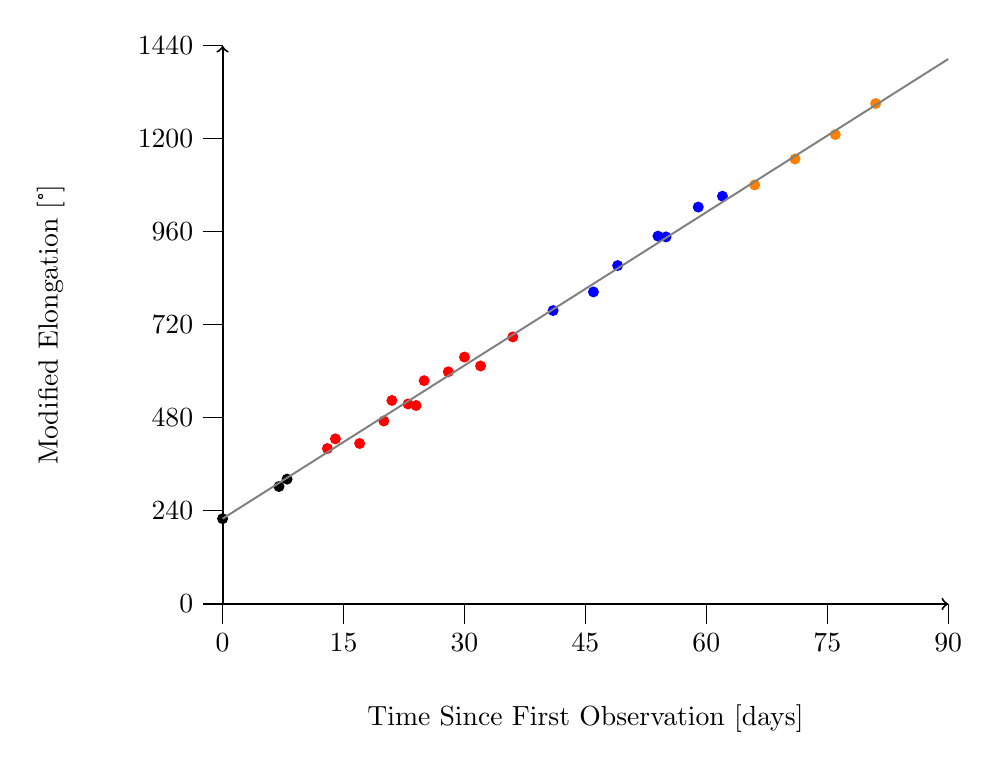
\begin{tikzpicture}
\draw[black, line width=0.25mm, ->] (0.0,0) -- (0.0,{\linewidth*0.76*0.7692});
\draw[black, line width=0.25mm, ->] (0.0,0) -- (\linewidth*0.76,0);
\draw[black] (0,0) -- ++(0.0,-0.25) node[below] {0};
\draw[black] ({15.0/90.0*\linewidth*0.76},0) -- ++(0.0,-0.25) node[below] {15};
\draw[black] ({30.0/90.0*\linewidth*0.76},0) -- ++(0.0,-0.25) node[below] {30};
\draw[black] ({45.0/90.0*\linewidth*0.76},0) -- ++(0.0,-0.25) node[below] {45};
\draw[black] ({60.0/90.0*\linewidth*0.76},0) -- ++(0.0,-0.25) node[below] {60};
\draw[black] ({75.0/90.0*\linewidth*0.76},0) -- ++(0.0,-0.25) node[below] {75};
\draw[black] ({90.0/90.0*\linewidth*0.76},0) -- ++(0.0,-0.25) node[below] {90};
\draw[black] (0.0,0) -- ++(-0.25,0) node[left] {0};
\draw[black] (0.0,{240.0 / 1440.0*\linewidth*0.76*0.7692}) -- ++(-0.25,0) node[left] {240};
\draw[black] (0.0,{480.0 / 1440.0*\linewidth*0.76*0.7692}) -- ++(-0.25,0) node[left] {480};
\draw[black] (0.0,{720.0 / 1440.0*\linewidth*0.76*0.7692}) -- ++(-0.25,0) node[left] {720};
\draw[black] (0.0,{960.0 / 1440.0*\linewidth*0.76*0.7692}) -- ++(-0.25,0) node[left] {960};
\draw[black] (0.0,{1200.0 / 1440.0*\linewidth*0.76*0.7692}) -- ++(-0.25,0) node[left] {1200};
\draw[black] (0.0,{1440.0 / 1440.0*\linewidth*0.76*0.7692}) -- ++(-0.25,0) node[left] {1440};
\draw[black] ({-0.18*\linewidth},{0.5*\linewidth*0.76*0.7692}) node[rotate=90] {Modified Elongation [°]};
\draw[black] ({0.5*\linewidth*0.76},{-0.12*\linewidth}) node {Time Since First Observation [days]};
\fill[black] ({0/90.0*\textwidth*0.76},{220/1440.0*\textwidth*0.76*0.7692}) circle (0.07);
\fill[black] ({7/90.0*\textwidth*0.76},{303/1440.0*\textwidth*0.76*0.7692}) circle (0.07);
\fill[black] ({8/90.0*\textwidth*0.76},{322/1440.0*\textwidth*0.76*0.7692}) circle (0.07);
\fill[red] ({13/90.0*\textwidth*0.76},{401/1440.0*\textwidth*0.76*0.7692}) circle (0.07);
\fill[red] ({14/90.0*\textwidth*0.76},{426/1440.0*\textwidth*0.76*0.7692}) circle (0.07);
\fill[red] ({17/90.0*\textwidth*0.76},{414/1440.0*\textwidth*0.76*0.7692}) circle (0.07);
\fill[red] ({20/90.0*\textwidth*0.76},{472/1440.0*\textwidth*0.76*0.7692}) circle (0.07);
\fill[red] ({21/90.0*\textwidth*0.76},{525/1440.0*\textwidth*0.76*0.7692}) circle (0.07);
\fill[red] ({23/90.0*\textwidth*0.76},{516/1440.0*\textwidth*0.76*0.7692}) circle (0.07);
\fill[red] ({24/90.0*\textwidth*0.76},{512/1440.0*\textwidth*0.76*0.7692}) circle (0.07);
\fill[red] ({25/90.0*\textwidth*0.76},{576/1440.0*\textwidth*0.76*0.7692}) circle (0.07);
\fill[red] ({28/90.0*\textwidth*0.76},{599/1440.0*\textwidth*0.76*0.7692}) circle (0.07);
\fill[red] ({30/90.0*\textwidth*0.76},{637/1440.0*\textwidth*0.76*0.7692}) circle (0.07);
\fill[red] ({32/90.0*\textwidth*0.76},{614/1440.0*\textwidth*0.76*0.7692}) circle (0.07);
\fill[red] ({36/90.0*\textwidth*0.76},{689/1440.0*\textwidth*0.76*0.7692}) circle (0.07);
\fill[blue] ({41/90.0*\textwidth*0.76},{757/1440.0*\textwidth*0.76*0.7692}) circle (0.07);
\fill[blue] ({46/90.0*\textwidth*0.76},{805/1440.0*\textwidth*0.76*0.7692}) circle (0.07);
\fill[blue] ({49/90.0*\textwidth*0.76},{873/1440.0*\textwidth*0.76*0.7692}) circle (0.07);
\fill[blue] ({54/90.0*\textwidth*0.76},{949/1440.0*\textwidth*0.76*0.7692}) circle (0.07);
\fill[blue] ({55/90.0*\textwidth*0.76},{947/1440.0*\textwidth*0.76*0.7692}) circle (0.07);
\fill[blue] ({59/90.0*\textwidth*0.76},{1024/1440.0*\textwidth*0.76*0.7692}) circle (0.07);
\fill[blue] ({62/90.0*\textwidth*0.76},{1052/1440.0*\textwidth*0.76*0.7692}) circle (0.07);
\fill[orange] ({66/90.0*\textwidth*0.76},{1081/1440.0*\textwidth*0.76*0.7692}) circle (0.07);
\fill[orange] ({71/90.0*\textwidth*0.76},{1148/1440.0*\textwidth*0.76*0.7692}) circle (0.07);
\fill[orange] ({76/90.0*\textwidth*0.76},{1211/1440.0*\textwidth*0.76*0.7692}) circle (0.07);
\fill[orange] ({81/90.0*\textwidth*0.76},{1291/1440.0*\textwidth*0.76*0.7692}) circle (0.07);
\draw[gray, line width=0.25mm] (0,{220/1440.0*\linewidth*0.76*0.7692}) -- (\linewidth*0.76, {(90.0 / 27.321661 * 360.0 + 220.0) / 1440.0*\linewidth*0.76*0.7692});
\end{tikzpicture}
\caption{\label{fig:days_mod_elongation_with_trend}The graph of the modified elongation by time since the first observation with a trend line shown. The points are color coded to help identify the points in each graph.}
\end{subfigure}
\caption{Graphs of elongation or modified elongation with time. Fig \ref{fig:days_elongation_data_only}, using the raw elongation data, shows a sawtooth pattern because the elongation `wraps around' from 359° back to 0°. The elongation is therefore modified to show the overall trend, adding 360° every time that the elongation would wrap back to 0°. This modified elongation and the resulting trend are shown in Figures \ref{fig:days_mod_elongation_data_only} and \ref{fig:days_mod_elongation_with_trend}.}
\end{figure}

Instead of using the calculated elongation, however, increase the number by $360^\circ$ for every time that the elongation `falls back' to zero.  For example, using the data from Table \ref{Tab:elongation}, the resulting modified elongations (i.e. that with extra multiples of $360^\circ$) are shown in Table \ref{Tab:mod_elongation}.\\

Fig. \ref{fig:days_mod_elongation_data_only} shows a graph with the data using modified elongation. The results show a linear trend, where elongation is increasing with (nearly) every observation. If you find that one of your data points lies well above or below the trend, it is likely because you unnecessarily added 360° or more, or didn't add 360° when you needed to. For these values, add or subtract 360° as needed until the data better matches the overall trend.


After you have made a graph, you should see a linear trend. Using a straight edge and a pencil or pen, draw a line through the data that best matches the trend. The line should have about half of all the data points above it, and about half below. Fig. \ref{fig:days_mod_elongation_with_trend}. Using the line, find the elongation value when the line is at 0 days, and the elongation value when the line is on the last day of your observations. Calculate the slope of the line by:

\BE \mathrm{Slope} = ((\mathrm{Elongation~of~line~on~last~day}) - (\mathrm{Elongation~of~line~at~0~days})) \div (\mathrm{Number~of~days}). \EE

In the obervation examples above, the line may be at $220^\circ$ on day 0, and $1250^\circ$ on day 78. The slope is then $(1250^\circ - 220^\circ) \div 78~\mathrm{days} = 13^\circ / \mathrm{day}$.\\
\begin{table}[!h]
\centering
\begin{tabular}{|c|c|c|c||c|c|c|c|}
\hline
 		& Time 			&   			&   			&  		& Time 			&   			& 				\\
 		& since 		&   			&   			&  		& since 		&   			& 				\\
 		& first  		&   			& Modified		&		& first  		&   			& Modified		\\
 		& observation  	& Elongation  	& Elongation	&		& observation  	& Elongation  	& Elongation	\\
Date 	& (days) 		& (°)  			& (°) 			& Date 	& (days) 		& (°)  			& (°)			\\
\hline
Dec 26 & 0 & 220 & 220 & Jan 27 & 32 & 254 & 614\\
Jan 02 & 7 & 303 & 303 & Jan 31 & 36 & 329 & 689\\
Jan 03 & 8 & 322 & 322 & Feb 05 & 41 & 37 & 757\\
Jan 08 & 13 & 41 & 401 & Feb 10 & 46 & 85 & 805\\
Jan 09 & 14 & 66 & 426 & Feb 13 & 49 & 153 & 873\\
Jan 12 & 17 & 54 & 414 & Feb 18 & 54 & 229 & 949\\
Jan 15 & 20 & 112 & 472 & Feb 19 & 55 & 227 & 947\\
Jan 16 & 21 & 165 & 525 & Feb 23 & 59 & 304 & 1024\\
Jan 18 & 23 & 156 & 516 & Feb 26 & 62 & 332 & 1052\\
Jan 19 & 24 & 152 & 512 & Mar 02 & 66 & 1 & 1081\\
Jan 20 & 25 & 216 & 576 & Mar 07 & 71 & 68 & 1148\\
Jan 23 & 28 & 239 & 599 & Mar 12 & 76 & 131 & 1211\\
Jan 25 & 30 & 277 & 637 & Mar 17 & 81 & 211 & 1291\\
\hline
\end{tabular}
\caption{\label{Tab:mod_elongation}Same as Table \ref{Tab:elongation} but with modified elongation included.}
\end{table}


Finally, divide $360^\circ$ by the slope, and you will find the period of the Moon's orbit:
\BE \mathrm{Period} = 360^\circ \div (\mathrm{Slope}). \EE

Using the example above, it is $360^\circ \div 13^\circ / \mathrm{day} = 28~\mathrm{days}$.

You may use a spreadsheet such as Microsoft Excel / Office or LibreOffice Calc / Office, or any other graphing software to create the graph and the trend line; however, \textbf{do not show the equation on the chart}. You should instead describe the trend in the text of your write-up.

\section{Relation between elongation and phase}
To find / demonstrate the relation between phase and elongation, create a graph with elongation (not modified elongation) as the horizontal axis and phase number as the vertial axis. As you did for the days and elongation plot, draw a line that shows the trend in the data. In your write up, show this graph, and describe the relation that you see. i.e. when the elongation is 0, what is the phase? When the elongation is $180^\circ$, what is the phase?

%\section{Finding the length of day (optional)}
%Finding the length of the day requires good observations and sketches. It could be very challenging, so it is an optional part of this project.

%To find the length of the day on the Moon, you need reasonably good sketches that show features on the Moon. Make sure to capture the same features on all or most observations. It will be slightly easier to do this during nighttime observations rather than those that you take during the day. You may attempt to use the camera on your phone, or a nicer camera if you have one, to try to take pictures of the moon and use these as the basis for your sketches. Note that your phone camera may have trouble with overexposure.

%To find the length of the day on the Moon, pick a specific point on a specific feature. From your observations when the Moon's phase is waning, make note of when you can see the terminator (the line between light and dark) near the feature while it is illuminated. A few days later, when the feature is no longer illuminated, estimate the day on which the feature switched from illuminated to dark. A couple of weeks later, when the Moon is waxing, pay attention to when the feature is still dark, then when you are first able to see the feature. Again, estimate the day on which the feature switched from dark to light. 

%Once you have completed your analysis between phase and elongation, and of the period of the Moon's orbit; estimate the length of time in days that the feature is illuminated, and the length of time in days that the feature is dark. The length of day is the sum of the illuminated time and the dark time.

%In the write up, provide some description of your observations. You may wish to include one or two sketches or images. You should answer the following questions:
%\begin{itemize}
%\item Does the Moon have observable rotation from the Earth? i.e. Do the features always appear in the same place,? Do you see different features at different times of the month or in different places?
%\item How long is a day on the Moon? i.e. how long is a particular point illuminated?
%\end{itemize}

\section{Graphs in scientific documents}
When generating a graph for use in a scientific document, there are a few things to keep in mind.
\begin{itemize}
\item The purpose of a graph is to demonstrate a trend (or lack of trend) in the data. If there is a trend, the reader should be able to see the trend and predict a value on the vertical axis based on some choice of a value on the horizontal axis.
\item The data should almost always be presented as a scatter plot. There are occasions when a bar graph or pie chart are used, but these are relatively rare (at least in astronomy).
\item The data in the plot should not be connected by lines or curves.
\item A trend may be included in the plot (a line or other appropriate mathematical function) but the equation for the trend should not be listed on the graph.
\item A legend should not be included if there is only one set of data.
\item There must be a axis title and a description of the units used for each axis.
\item Each axis should have multiple numeric labels, preferably three or more.
\item The graph itself should not have a title.
\item Make sure that the horizontal axis is a variable, not a label.
\end{itemize}
\end{document}
